%
\documentclass[11pt]{article}
\usepackage{amssymb}
\usepackage{amsmath}
\usepackage{amsthm}
\usepackage{pst-all}
\usepackage{newicktree}
\usepackage{graphicx}
\usepackage[left=1.4in,right=1.4in,top=1in,bottom=1in,includeheadfoot]{geometry}
\usepackage{setspace}
\usepackage{natbib}

\newtheorem{theorem}{Theorem}
\newtheorem{corr}{Corollary}
\newtheorem{assumptions}{Assumptions}
\newtheorem{definition}{Definition}

\DeclareMathOperator*{\argmax}{arg\,max} 

\frenchspacing
\linespread{1.25}
\parskip= 2 pt

\title{Foundations of the Age-Area Hypothesis \\ \large{Preliminary and Incomplete - Not for Citation}}
\author{\textbf{Matthew J. Baker} \\ Department of Economics \\ Hunter College and the Graduate Center, CUNY}

\begin{document}

\maketitle
\begin{abstract}
\noindent A commonly-used tool in explaining the origins, geographical dispersion, and degree of relatedness between cultures is the Age-Area Hypothesis developed by \cite{sapir16}. The hypothesis posits that the origin point of a group of related cultures or a linguistic stock is most likely where the languages comprising the stock are most divergent. While compelling and often-corroborated, the Age-Area Hypothesis has never been founded in basic principles, and this lack of structure limits its use. I describe a micro-founded model of the Age-Area Hypothesis based on mass migration, develop a measure of divergence between cultures based on phylogenetic trees, and develop an Age-Area Theorem. The model allows computation of probabilities that different locations are the origin points for the constituents of a group of related cultures. The model also provides a probabilistic explanation of Occam's razor: migratory paths explaining the geographical dispersion of related cultures that are simpler are  more likely. The paper concludes with applications to the origins of the Na-Dene and Afro-Asiatic Ethno-linguistic groups. 
\end{abstract}
\newpage

\section{Introduction}
Studying the impact of ethnic, genetic, and cultural diversity on economic outcomes has become a central part of economics. \cite{ashraf13}, for example, discuss the nuanced role that genetic diversity might play in driving modern economic outcomes, while \cite{spolaore09} describe the importance of genetic distance and economic distance between populations. 

As \cite{cavalli95} have pointed out, genetic, ethnic, linguistic, and cultural diversity are all closely related, and much recent economic research (reviewed in \cite{alesina05}) has focused on the relationship between ethnic diversity, fractionalization and economic growth. Some research, such as \cite{spolaore13}, develops a link between ancient institutions and cultural practices on modern economic outcomes. 

Other work has pushed this agenda in a different direction, with the aim of understanding the origins of ethnolinguistic and genetic diversity around the world.   \cite{michalopoulos12} shows that geographical diversity is an important determinant of human diversity.  \cite{ahlerup12} develop a model of ethnic diversity based on genetic drift and migration. They show that, over time, populations spread out and experience cultural drift, and that populations that have been in place longer tend to be more culturally diverse. This echoes a long and rich tradition in other disciplines, as detailed in  \cite{mace05}. 

A - perhaps ``the'' - key contributor to the world-wide distribution of cultures are historical, large-scale mass migrations. And a critical tool in understanding the timing and sequence of events behind mass migrations is the so-called Age-Area Hypothesis (henceforth AAH). A leading early development and application of the idea is \cite{sapir16}, in his study of the geographical origins of the North American Na-Dene language group. The AAH is often invoked when linguistic evidence is used to develop or support hypotheses about where groups of related  cultures originated, how they evolved over time, and how the current geographical distribution of the cultures came to be.\footnote{One must be careful in invoking ``the'' AAH, as there are possibilities for confusion with other, sometimes unrelated, ideas. The AAH in this paper is not to be confused with, for example, the Sapir-Whorf Hypothesis, which refers to the idea that peoples' thinking is influenced by the structure of their language. What might be called the Cultural Age-Area Hypothesis is the principle that the more widely geographically distributed a cultural trait is, the older it likely is. } The AAH provides a critical link between geography and linguistic phylogenies. While one can find competing and sometimes contrary definitions in the literature, briefly stated, the hypothesis says that the geographic area where a phylogeny originated is most likely the place where the component languages of the phylogeny are most divergent, or maximally differentiated.

Applications - either implicit or explicit  - abound. \cite{atkinson03}, following \cite{renfrew87} hypothesis and \cite{dogolpolsky88}, couple computational linguistics with the AAH to suggest that the Indo-European languages originated in Anatolia, not, as has sometimes been argued, on the steppes of Siberia. \cite{ruhlen94} uses the AAH and also provides overviews of debates about the origins of the Na-Dene cultures, the Bantu expansion in Africa, and the peopling of the South Pacific. \cite{ehret01} Makes extensive and efficient use in hit sweeping account of how and when the cultures of Africa found their current locations.

In spite of its widespread invocation, there is, to my knowledge, no theoretical basis for the hypothesis. The lack of a theoretical basis for the  AAH is a problem not only because it leads to imprecise definition, but also because it is difficult to use in technical situations. Suppose one wished to include a migratory path in a statistical model of migration and cultural evolution, or that one wanted to integrate the timing and path of migration into a larger statistical model, perhaps with an eye toward more accurately controlling for relatedness between differing peoples. Since the hypothesis has no theoretical underpinnings, it is difficult to see how to construct a likelihood for a certain path or migratory history, or even for the likelihood of competing hypotheses.

I develop a theoretical foundation for the age-area hypothesis. The model is micro-founded in the sense that it can be based on microeconomic principles and an associated back story. The theory shows how probabilities that different locations as being the point of origin and Occam's razor are interdependent. That is, it turns out that migratory histories that are simpler in a well defined sense are also more likely. The model indicates that migratory paths that originate at deeper points in a phylogenetic tree can be thought of as simpler in a very precise fashion, in that inclusion of such paths in a migratory history also results in a model with fewer parameters. These ideas also lead to a particular definition of divergence or dissimilarity for each constituent culture in the phylogeny. 

I then develop an Age-Area Theorem using these ideas. The theorem presents assumptions under which a culture that is more linguistically divergent from the others in the stock is also more likely to reside at the point of origin of the stock. I then present a computational algorithm which relies upon backwards traversal of a phylogenetic tree, along with some extensions of the model. I conclude by discussing some applications. The theorem, when applied recursively, also yields what can be construed as a maximum-likelihood migratory path. 

It is worth emphasizing that the model can be used to formulate an likelihood function for migratory patterns, and hence can be included as part of a larger estimation problem. Maximum likelihood methods are commonly used in linguistics to estimate linguistic divergence times. So, using the results of this paper, one could in principle estimate or include the implied migratory path as part of a larger phylogenetic estimation problem. Likelihood methods are also amenable to Bayesian techniques, which expand estimation possibilities tremendously, and provide an avenue for including archaeological and genetic evidence in estimation as well. 

\section{Background Literature}

One of the dominant means of describing how closely-related cultures are is through language and linguistic drift, which turns out to be a fairly reliable guide to how far in the past two similar cultures began to drift apart after some event - often a large-scale migration - lead to their geographical separation. The AAH is a primary tool linking geography with cultural drift. \citet[p.12]{trask00} attributes the (Linguistic) Age-Area Hypothesis - also called the center-of-gravity principle, the genetic diversity principle, and Sapir's principle - to the work of \cite{latham51}  and \cite{sapir16}. \cite{trask00} further notes that \cite{mallory97} and \cite{nichols97} have employed and qualified the AAH in various ways.   \citet[p.336]{dimmendaal11} expresses some doubts about the exact origins of the AAH, referring to it as the ``principle of least effort,'' while noting that ``This principle probably was applied first by the scholars working on Amerindian Languages, e.g. \cite{sapir16} and \cite{dyen56}''.

In what seems to be the initial application of the idea, \cite{sapir16} writes:

\begin{quote}
 As is well known, [Athabaskan] languages are spoken in three geographically isolated areas, a very large northern area (interior of Alaska to near Hudson Bay), a Pacific area (southwestern Oregon and Northwestern California), and a southern area (Arizona, New Mexico, and western Texas)...it would seem that the historical center of gravity lies rather in the north than in either of the other two regions and that the occupation of these latter was due to a southward movement of Athabaskan-speaking tribes. It is important to observe that the argument is not in any way dependent on the fact that the northern tribes cover a much vaster territory that those of the other two groups or even directly on the fact that probably a larger number of distinct dialects are spoken in the north than elsewhere. The argument for the northern provenience of the Athabaskan tribes is clinched by a further linguistic fact, namely that the Athabaskan dialects from one of the three major divisions of the Na-dene stock, the other two being Haida and Tlingit. The fact that the latter are spoken in the northwest coast area so emphatically locates the historical center of gravity of the stock in the north that it becomes completely impossible to think of the Athabaskan tribes as having spread north from California or the southwest. 
\end{quote}


\citet[p. 623]{dyen56} also cites this passage, and goes a bit further in cleaning up the theory and defining how things work in practice, describing concepts such as migrations and even stating two basic postulates to be employed in assessing homelands for linguistics. Her first postulate is that the area of origin of related languages is continuous. The second postulate, which is more important for the purposes of this paper, is that ``the probabilities of different reconstructed migrations are in inverse relation to the number of language movements that is required.'' \citep[p.613]{dyen56} 
To some degree, my principle objective in this paper is to clarify and develop Dyen's second postulate, rather than simply asserting that it is true.

As a final note, consider some of the comments made in \cite{greenhill05}, who discuss the peopling of the South Pacific and also present a detailed discussion of quantitative methods in historical linguistics. They develop statistical tests comparing different hypotheses for how the South Pacific came to be settled. They write the following in describing the need for formal modeling and associated hypothesis tests in resolving disputes about migratory routes:

\begin{quote}
``...many expansion scenarios are little more than plausible narratives. A common feature of these narratives is the assertion that a particular line of evidence (archaeological, linguistic, or genetic) is `consistent with' the scenario. `Consistent with' covers a multitude of sins. Rigorous tests require a measure of exactly how well the data matches the proposed scenario. They also require an explicit evaluation of alternative hypotheses. ...a framework for the rigorous evaluation of these hypotheses is clearly desirable. \citep[p. 31]{greenhill05} 
\end{quote}
This statement could easily have been written in describing the reason for the current paper, which creates a method for considering a family of dispersal hypotheses that flow naturally from statement of the model.

 


\section{Problem Description and Motivation}

Consider the hypothetical phylogenetic tree displayed in figure \ref{fig1}. For clarity, the figure depicts the phylogenetic relationship between cultures, which has perhaps been obtained through a careful analysis of the languages of the cultures so that one can deduce the times at which the cultures seem to have separated. $A$ is evidently the most divergent culture in that the last time at which the cultures had a common ancestor is further in the past than it is for any of $B$, $C$, $D$, or $E$, all of whom are closer relatives to one another. $D$ and $E$ are the most closely related cultures. To avoid forming impressions based on evidence that is not part of the hypothesis, we will suppose that the locations of the
groups have been concealed from us, and that we have no access to archaeological or historical information about the constituent cultures of the phylogenetic tree came to be in their current locations.

The AAH asserts that the geographical origins of this cultural group is $A$'s current location, as $A$  is, the most divergent culture (speaker of the most divergent language, that is) from the group. Recursive application of the AAH would lead one to a most likely migratory route: the stock originated at A's location. There was then a migration from $A$'s location to $B$'s location, then from $B$ to $C$, and then from $C$ to either $D$ or $E$.  

\begin{figure}
\begin{center}
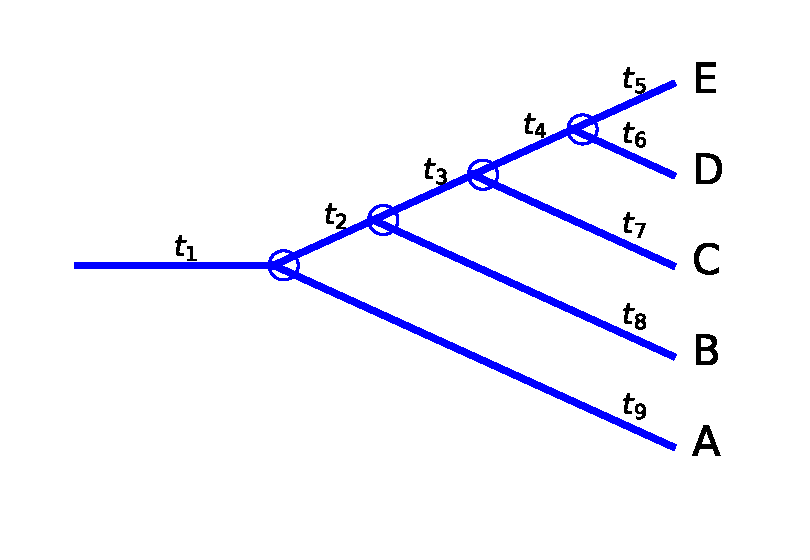
\includegraphics[width=\textwidth]{AncillaryFiles//figure1.eps}
\caption{A Phylogenetic tree} \label{fig1}
\end{center} 
\end{figure}

Why would one believe this was the most likely explanation for how the cultures came to be where they are?\ There are a number of other possible routes, even though the phylogenetic tree constrains the possibilities. For example, it can never be the case that a migration from D to E preceded one from D to C; this would be inconsistent with the observed linguistic drift over time. But another possible  sequence of migratory events would be for an initial migratory episode from C to A, followed by another from C to B, followed by yet another migration from C to D or E.

\begin{figure}
\begin{center} 
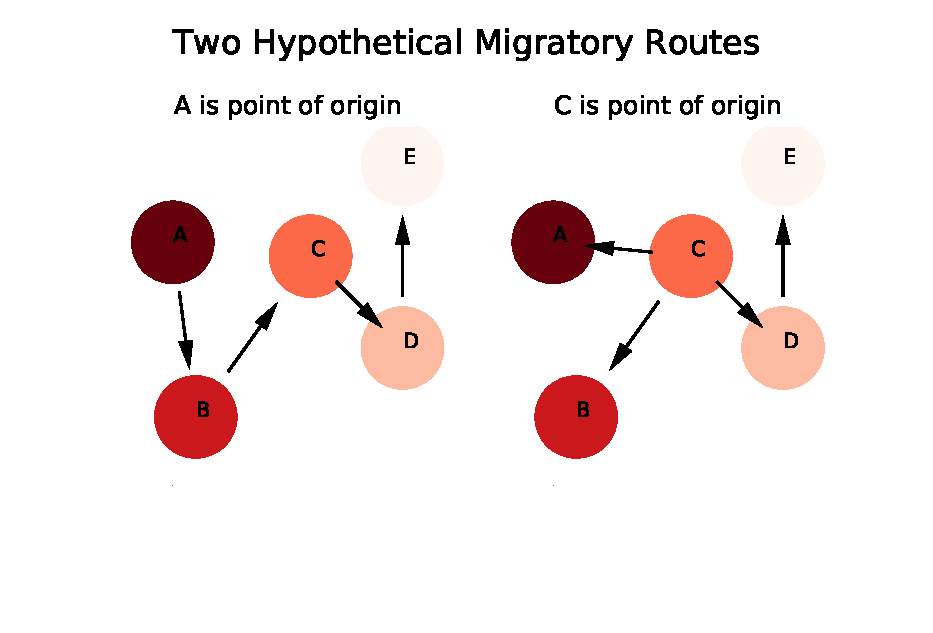
\includegraphics[width=\textwidth]{AncillaryFiles//figure2.eps} 
\caption{Potential migratory routes among a language stock consisting of five groups, following the Phylogenetic Tree in figure.} \label{fig2}
\end{center} 
\end{figure}

These two possible migratory routes are presented in figure \ref{fig2}, and the AAH asserts that the right-hand sequence is a less-likely migratory history than that on the left. Why? One might simply appeal to Occam's razor - the events on the left-hand side of figure \ref{fig2} require only one migratory chain, while the events on the right-hand side require three separate expansions: an initial migration from A to C, followed by another from A to B. A third migratory event is sufficient to take care of the last two groups: it begins from C continues to D, and then to E. Also clear from this example is the limited usefulness of positing a minimal number of moves to explain migrations. The above paths both require only four distinct population movements.  



We can now pose our question as follows: if we believe migratory events to be rare, and we wish to conserve them in explaining historical migrations, what sort of model would accomplish this? But can one make this operational in a more formal setting? Can one characterize parsimony in a meaningful mathematical and probabilistic way? 

\section{A model}

\subsection{Tree Basics}

I assume throughout that the entire phylogenetic tree is known, so the universe of migratory events that needs to be explained is observed. The tree can be constructed by any number of methods.\footnote{See, for example, \citet{nichols97} for a survey of methods.  } I also assume the tree is a full, rooted, binary tree, meaning that there is a single origin node and branch, all other nodes have a single parent, all interior nodes have exactly two children, and all terminal nodes have zero children. 

A binary tree with $n$ taxa or leaves has $n-1$ internal nodes. The tree in figure \ref{fig1}, for example,  has five terminal nodes/taxa  and four internal nodes. This also applies to subtrees, which means that if a node has $k$ successors (children and childrens' children, etc.), then it is followed by $k-1$ nodes.

\subsection{Migratory Chains}
 
I build the model around \textit{migratory chains}, which can be thought of as sequences of \textit{migratory events}, similar to the way in which they are defined in \cite{dyen56}. A migratory chain is manifest on a phylogenetic tree as a directed path from the root of a tree (or subtree) to a terminal node. Geographically, a migratory event corresponds with a movement of a population to a new geographical location, with a migratory chain being composed of a sequence of such movements unfolding over time.\footnote{For the time being, I posit that a migratory event is an instantaneous jump to a new location. I will discuss this further below.}

 I call a  collection of migratory chains that span the entire phylogenetic tree a \textit{migratory history}. Hypothesizing that a particular culture or society is the point of origin of the tree amounts to positing some sequence of migratory chains through the phylogenetic tree, of which the deepest chain starting from the root starts from the point of origin. I assume that a migratory chain has the following properties.

\begin{assumptions}{Migratory Chains}    
\begin{enumerate}
\item Each migratory chain occupies a single location at any given point in time.
\item When a chain moves from its current location, a new chain starts in its place at the given location.
\item Migratory chains move at random times according to an exponential density.
\item Each migratory chain is distinct in that it has its own parameterized probability density.
\end{enumerate}
\end{assumptions}
I will call a migratory history originating at location $k$ $H_k$, and will assume that candidate migratory histories require the minimal number of migratory events or moves to explain the current distribution of the member cultures of a phylogeny. In the time dimension, a migratory chain is then a directed path through a sequence of nodes to a leaf node, and in space, a migratory chain appears at a sequence of jumps at randomly distributed times. Collectively, chains comprise a history if the tree is covered by chains. I\ denote the component chains of a history as $C_{jk}$.

\textit{Any} history employing the minimum number of moves will need exactly $n-1$ migratory events to span the tree. The events depicted in figure \ref{fig2} following from the tree in figure \ref{fig1} has 4 arrows between nodes, which corresponds with the number of migratory events required. This will be true regardless of where the migratory history is started. 

Each location where a society or culture represented by a terminal node resides,  $k=1,2,3,\hdots K;$ can be associated with a set of migratory histories $\mathcal{H}_k$. The previous statement accentuates the fact that there is typically more than one migratory history that is possible from origin point $k$. Each migratory history has some count of the total number of migratory chains required, which I refer to as  $N(H_k$). For the example on figure \ref{fig2}, the first history $N(H_a)=1$, while for the second, $N(H_c)=3$.    I also define a counting function for specific migratory chains as $n(C)$, which counts the number of migratory events in the chain, which is also a count of the nodes spanned by the given chain. 

These ideas can be applied to develop a likelihood associated with any particular history, and a related measure of divergence which I\ refer to as ``Dyen Divergence.' The Dyen Divergence relates phylogenetic distance and probability precisely, so I  can state and prove an `Age-Area Theorem' that relates  migratory histories, counts of migratory chains, counts of events in each chain, and likelihood. Parsimony or Occam's razor suggests that simpler explanations - those with smaller values for $C$'s - have higher probabilities and this is in indeed true under Assumptions 1, owing to the shape of the exponential distribution, as I now show in a preview of the logic used to state the theorem.
 I  develop a comparison of the two scenarios described in figures \ref{fig1} and \ref{fig2} within the confines of the model. Let the likelihood that $k$ is the point of origin be denoted by $L_k$. I begin by assuming that we do not know the exact times at which branching events occur, but instead only know the basic structure of the tree. The points can be treated as known but can be `integrated out' by replacing the Exponential model with a Poisson model. 

The first migratory history described on figure \ref{fig2} requires an initial migratory chain to start at the root of the tree, which then proceeds from location $A$ to $B$, then from $B$ to $C$ and then finally to $D$ or $E$.\footnote{In the next subsection, I will describe a more intricate example in which a decision must be made among multiple possibilities.} But each time the migratory chain proceeds to a new location, by Assumption 1, a new one starts in its place. Importantly, in the example in figures \ref{fig1} and \ref{fig2}, these new chains never create any new migratory events and only lead to terminal nodes of the tree. 

The probability of observing this sequence of events can be written by combining the densities of the components of  $H_A$, which I\ can write as:\footnote{Throughout I shall use numbers to denote interior branches and nodes along a tree, and the labels of endpoints to denote the terminal branches of the tree.}
\begin{equation*}
L_A=\textrm{Prob}(H_A)=P(C_{1A})P(C_{AA})P(C_{BA})P(C_{CA})P(_{DA})
\end{equation*}
Using the form of the distribution for the chains, I have:
\begin{equation} \label{e1}
L_A = \frac{(\lambda_1 T)^4e^{-\lambda_1T}}{4!}\frac{(\lambda_2 t_6)^0e^{-\lambda_2t_6}}{0!}\frac{(\lambda_3 t_7)^0e^{-\lambda_3t_7}}{0!}\frac{(\lambda_4 t_8)^0e^{-4t_8}}{0!}
\end{equation} 

Equation (\ref{e1}) is perhaps more expansive than necessary, as all the terms raised to the $0$th power are degenerate. The probability in equation (\ref{e1}) could also be written as:
\begin{equation} \label{e2}
L_A = \frac{(\lambda_1 T)^4e^{-\lambda_1T}}{4!}e^{-\lambda_2t_6}e^{-\lambda_3t_7}e^{-\lambda_4t_8}
\end{equation} 
The log-likelihood associated with equation (\ref{e2}) is:
\begin{equation} \label{e3}
\ln L_A  = 4\ln(\lambda_1 T) -4\lambda_1T-\ln(4!)-\lambda_2t_6-\lambda_3t_7-\lambda_4t_8
\end{equation} 
What values of $\lambda_i$ maximize the likelihood in (\ref{e3})? As alluded to above, $\lambda_2=\lambda_3=\lambda_4=0$ at the optimum. Since these chains never go further than their current locations, the maximum likelihood estimate suggests that they are degenerate with rate parameter equal zero. 

The derivative of (\ref{e3}) with respect to $\lambda_1$, however, generates a meaningful parameter estimate. Differentiating with respect to $\lambda_1$ and solving the first-order condition gives $\lambda_1^*=\frac{4}{T}$. Substituting this and other optimal values back into the objective function gives the (concentrated) likelihood $L_A$ as:
\begin{equation}  \label{l3}
L_A=\frac{4^4e^{-4}}{4!}
\end{equation}

Equation (\ref{l3}) is that it reflects that only one non-degenerate migratory chain is needed to explain the whole tree, given that the migratory history starts at $A$. In this sense, this a parsimonious explanation for the current distribution of cultures. 

Contrast this with the case in which $C$ is posited to be the origin point. To maintain consistency with the phylogeny, the requirements are:  1) a migratory chain starting at $C$ leading to $A$, 2) another migratory chain starting at $C$ going to $B$, and then 3) a migratory chain that starts at $C$ and proceeds to $D$ (or $E$) and then finally to $E$ (or D). Degenerate chains start at location $C$ and $D$ (or $E$). According to the model, each of these chains requires its own Poisson/Exponential parameter, which, omitting degenerate chains, gives:
\begin{equation} \label{l4}
L_{C}=\frac{(\lambda_1t)^1e^{-\lambda_1t}}{1!}\frac{(\lambda_2(t-t_0))^1e^{-1}}{1!}
\frac{(\lambda_3(t-t_0-t_1))^2e^{-\lambda_3(t-t_0-t_1)}}{2!}
\end{equation} 
Maximizing $L_{}_{C}$ in (\ref{l4}) with respect to $\lambda_1,\lambda_2$ and $\lambda_3$, and substituting the result back into the right-hand side of (\ref{l4}) gives:
\begin{equation} \label{l5}
L_{C}=\frac{1^1e^{-}}{1!}\frac{1^{1}e^{-1}}{1!}\frac{2^2e^{-2}}{2!}=
\frac{2^2e^{-4}}{2!}
\end{equation} 

Suppose that the origin point was known to be one of these two locations. According to equation (\ref{l5}), the likelihood that $A$ is the point of origin relative to $C$ depends upon $L_{A} /(L_A+L_C)$; a race between the functions $\frac{4^4}{4!}$ and $\frac{2^2}{2!}$, so the relative probability  $A$ is the point of origin would then be 84\%. 

A key feature of the previous analysis is the function: 
\begin{equation*}
h(n)=\frac{n^n}{n!}
\end{equation*}
which is convex in $n$, which is in turn the notation I use for the count of the number of nodes contained in a migratory chain. This convexity, which owes to the structure of the Poisson-Exponential distribution, implies that one is better off with explanations that require fewer non-degenerate parameters, or, equivalently, more degenerate parameters, which have the effect of lumping migratory events into longer chains. Breaking up a migratory chain into two smaller chains eschews this convexity, and results in a less likely explanation. That is, for any  $k \in (1,n-1)$, it is true that:
\begin{equation*}
h(n) > h(n-k)h(k)
\end{equation*} 

This example illustrates the essentials of the model. 

\section{Divergence}
The biggest detail that needs to be worked out in support of the above argument is how migratory chains that are more parsimonious and therefore more likely relate to a measure of linguistic divergence. For any migratory history $H_k$, there will be some migratory chain that has the largest value of $n$, and accordingly, define:

\begin{equation*}
n_{H_k}^*=\max_{C_{ik} \in H_k} \{n(C_{1k}),n(C_{2k}),\hdots,n(C_{N(H_k)k)} \}
\end{equation*}
That is, $n^*_{H_{k}$ is the node count for the longest component chain of history $H_k$. The following couples this definition with the previously-introduced count of migratory chains to develop what I refer to as Dyen divergence, as \cite{dyen56} went far in developing the basic concepts. 


\begin{definition}{\textbf{Measures of Divergence}:}
Define a function for a migratory history $D_{H_{k}}=m(n^*_{H_k}$,N(H_k)).$ that is increasing in the first argument and decreasing in the second. Define the \textbf{Dyen Divergence} of culture $k$ in terms of the history $H^*_k$ as:
\begin{equation*}
D_k=\max \{D_{H_{1k}},D_{H_{2k}},\hdots D_{H_{Ik}} \}
\end{equation*}
\end{definition}

The above definition defines not `a' measure of divergence, but a family of such measures. The measure itself is a) increasing in the number of events associated with the largest chain in the history, and b) decreasing in the number of chains in the history. The largest such value is the Dyen Divergence of culture $k$. Using the probability functions and this measure of divergence, one can now show that larger divergences coincide with more likely chains.  


\section{ Age-Area Theorem}

\begin{theorem}[Age-Area Theorem]
Suppose that Assumptions 1 hold, and define Divergence as in definition 1. Then  
\begin{equation*}
D_k \geq D_j \Longrightarrow L_k\geq L_j
\end{equation*}
and in particular
\begin{equation*}
k=\argmax\left[D_1,D_2,D_3,\hdots,D_n\right] \Longrightarrow k=\argmax\left[L_1,L_2,L_3,\hdots,L_n\right]
\end{equation*}
\end{theorem}
\begin{proof}

The probability that $k$ is the point of origin is a product of the functions $h(n)$, which are convex in $n$,  the number of migrations covered by a migratory chain. Thus, if $C_i$ chains are required, the length of each are $N_i$, we may write:
\begin{equation*}
L_k \propto\prod_{j=1}^{N(H^*_k)} h(n_j)
\end{equation*} 
By the convexity of $h(N)$, and the fact that $\sum n_j=I$, where $I$ is the number of internal nodes of the phylogenetic tree, $L_k$ is maximized by the smallest number of chains, with the largest $n$. The second part of the theorem follows because any finite ordered set has a maximum in the set.  
\end{proof} 

The theorem is vague about the exact definition of divergence, but and suggests that any measure obeying the definitions 1, that is increasing in the number of chains and the length of the longest chain will do. One candidate would be the ratio of the two:
\begin{equation*}
D^1_i=\frac{n^*_{H^*_k}}{N(H^*_k)}
\end{equation*}
another candidate would be the difference:
\begin{equation*}
D^2_i=n^*_{H^*_k}-N(H^*_k)}
\end{equation*}



the measure of divergence could be constructed in many different ways so long as it is increasing in the length of the longest chain, and decreasing in the number of chains. The above-mentioned functions  are a measure that is easily constructed using any phylogenetic tree.  

\subsection{Additional Examples and Discussion}

 
\begin{figure}
\begin{center}
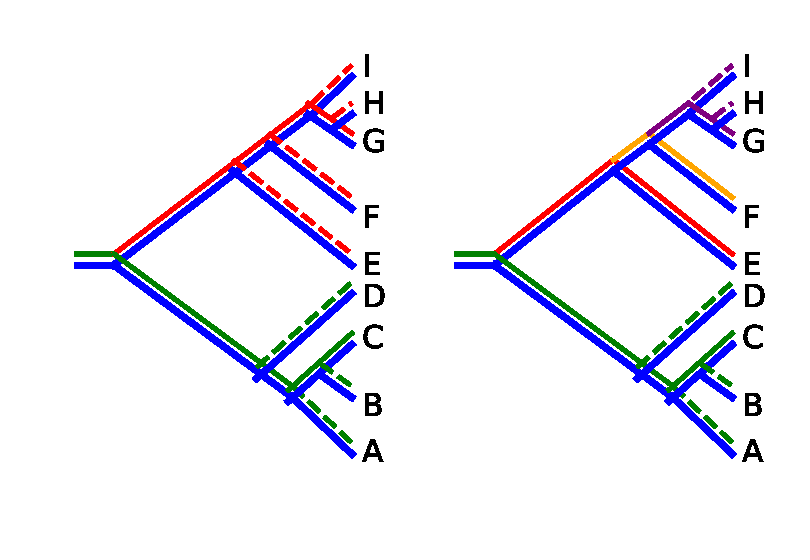
\includegraphics[width=\textwidth]{AncillaryFiles//example1.eps}
\caption{Two hypothetical migratory histories through a given Phylogenetic Tree. The picture on the left takes location $E$ as the point of origin, while that on the right takes point $I$ as the origin. } \label{ex1}
\end{center} 
\end{figure}

For a first example, in the phylogeny in figure 3, I have superimposed hypothetical migratory paths{} o a few different points of origin. The point of origin of the left-hand component figure is posited to be point $E$, which necessitates a migratory history with two migratory chains.  The first history starts at $E$ and goes to $D$'s location, and then from $D$'s location to $A$'s, from $A$'s to $B$'s, and finally from $B$'s to $C$. This history is traced out in green on the figure. A second migratory chain (traced in red) must then be invoked to explain the sequence of events leading to the upper half of the tree. This chain begins at $E$'s location again, and then moves on to $F$'s, then $I$'s, then $H$'s, and finally to $G$'s location. Under the model, the likelihood of this sequence of events is:

\begin{equation*}
L^*_E =  \frac{4^4e^{-4}}{4!}\frac{4^4e^{-4}}{4!} =\left(\rigth\frac{4^4}{4!}\right)^2e^{-8}
\end{equation*}

This reflects the two required, non-degenerate migratory chains to explain the sequence of events.  If we were to use divergence measure $D_1$, two chains are required, each of which has a maximal length of 4. Hence, $D^1_E=4-2=2$ and D^2_E=4/2=2$ as well.

If $I$'s location is  to be the point of origin, more migratory chains need to be invoked. The first chain is again traced out in green, mimicking the case in which $E$ is the point of origin. But to explain how a group got to point $E$ given $I$ was the starting point, we need a single migratory chain consisting of a sole migratory event. We also need another migratory chain to explain how a group got to point $F$. Finally, a fourth migratory chain going from $I$, and then to $H$, and finally on to $G$ is needed. The likelihood of these events is then:

\begin{equation*}
L^*_I =\frac{4^4e^{-4}}{4!}\frac{1^1e^{-1}}{1!}\frac{1^e^{-1}}{1!}\frac{2^2e^{-2}}{2!}=\frac{4^4}{4!}\frac{2^2}{2!}e^{-8}
\end{equation*} 

One finds that in this case, the measures of divergence are $D_I^1=1$, and $D^2_I
=0$. One can see in these examples the roles that convexity and degeneracy plays in driving differences in likelihood. One can also observe that it is not sufficient to pick the location from which the longest chain an be assembled, as both $E$ and $I$ admit chains of length 4. 
If one wished to compare hypotheses about the two points, one might use the relative likelihood; in this case, the probability that $E$ is the point of origin is $L^*_E/(L^*_I+L^*_E)
=.84.$ Of course, one would like to have a more rigorous method for computing likelihoods in every settings, and this is described in a subsequent section which presents a computational algorithm.  

 


\subsection{Known branch lengths}

If branch lengths are known, no difficulties are posed for the basic ideas of the model. All that happens is that exponential densities replace the Poisson densities. The chief technical assumption that is required in this instance is that none of the branch lengths are too short. To illustrate how the model changes, return to figure  \ref{fig1}. Now, with branch lengths treated as known, the likelihood is governed by a collection of exponential distributions:

\begin{equation} \label{b1}
P_A = \lambda_1^4e^{-\lambda_1T}\lambda_2^0e^{-\lambda_2t_6}\lambda_3^0e^{-\lambda_3t_7}\lambda_4 ^0e^{-4t_8}
\end{equation} 

While there are still degenerate branches, in that the probability in equation \ref{b1} is maximized where $\lambda_2=\lambda_3=\lambda_4=0$, now $\lambda_1^*=\frac{4}{T}$ maximizes the likelihood, so the profile likelihood becomes:

\begin{equation} \label{b2}
L_A=\left(\frac{4}{T}\right)^4e^{-4}
\end{equation}

The likelihood for $C$ is:

\begin{equation} \label{b3}
L_{C}=\lambda_1^1e^{-\lambda_1T}\lambda_2^1e^{-\lambda_2(T-t_1)}
\lambda_3^2e^{-\lambda_3(T-t_0-t_1)}
\end{equation}

The profile likelihood associated with equation (\ref{b3}) is 

\begin{equation} \label{b4}
\frac{1}{T}\frac{1}{T-t_1}\left(\frac{2}{T-t_1-T_2}\right)^2
\end{equation}

So, as before, we still have a basic race between a rapidly increasing denominator and a slower-decreasing denominator; in expression (\ref{b4}), the decreasing length of the branches spanned in the denominator fulfills the role of the factorial term in the denominator of the Poisson model. The danger for the age-area theorem is that the branches will be very small, which will lead to the denominator being very large. However, if we impose a minimum branch length on the branches, we get the same convexity of the concentrated function as before, so we have:

\begin{theorem}[Age-Area Theorem  - known branch lengths]
Suppose that Assumptions 1 hold, and define Divergence as in definition 1. Also, suppose that branches are not too short.  Then  
\begin{equation*}
D_k \geq D_j \Longrightarrow L_k\geq L_j
\end{equation*}
and in particular
\begin{equation*}
i=\argmax\left[D_1,D_2,D_3,\hdots,D_{K}\right] \Longrightarrow i=\argmax\left[L_1,L_2,L_3,\hdots,L_K\right]
\end{equation*}
\end{theorem}

\begin{proof}
Under the assumptions, the concentrated likelihood remains convex. Proceed as in the previous statement of the theorem.
\end{proof}

\section{Microeconomic foundations}

The previous sections have leaned on properties of the Exponential/Poisson distribution. What justifies the choice of this distribution? One would like a model in which migrations move forward probabilistically, but at the same time, the impetus for the migration resets or takes on a different character once the migration moves on. 

First, suppose that there is a discrete set of habitable locations, and suppose that a shock randomly occurs that applies to all currently unoccupied locations. This creates an abundance of resources at all unoccupied places throughout the system. The shock is such that a natural carrying-capacity parameter increases, but this extra carrying capacity can be exhausted. If the population ever reaches some barrier level $\overline{b}$\ at a particular location, the carrying capacity is exhausted and falls to a level  immediately reverts to a level of $\underline{K}$. Once the population has adjusted, a new value of $\overline{b}$ is drawn, a new shock emerges, and time continues on. 

The key thing is that there are now $\overline{b}$ people at a place where carrying capacity is $\underline{K}$. At this point in time, there are now a superabundance of people in the given area, and some mass of these people may migrate to a new location.\footnote{A parable: a people currently occupy an island with a population of friendly birds, who also populate some unsettled islands. While plump, these birds taste terrible. By accident, one day it is discovered that a spice on the island makes the birds palatable, leading to an abundance of food. Human population adjusts to the newfound resource, and while the birds are plentiful, there are no problems. But one year, an unusually good agricultural crop pushes the human population higher than it usually is. The additional population strains the bird population leading to a collapse. Half of the population leaves for a new island, where birds are still plentiful.}



According to an arbitrage condition, a segment of the population realizes that it could migrate to a new location where the birds are plentiful even if migration is costly, and finds it in its interests to do so given the localized collapse of the bird population. The population splits into a migratory group based on arbitrage, the migratory group randomly selects a new location, and emigrates.\footnote{The location does not actually have to be random. The minimum cost reachable location is in fact the best, as is discussed in the section on model extensions.} After this emigration, the remaining population embarks on the discovery of a new resource.



To make these ideas concrete,  and see how they explicitly relate to the Exponential distribution, imagine that income per capita depends upon a resource level and also the current number of inhabitants. That is, flow per capita income at a particular location is
\begin{equation}
y_t=f(n_t,\theta_t)
\end{equation} 
I imagine that $f(n,\theta)$ is bounded above at some reasonable level. Individuals gain utility from consumption $x_t$ and children $k_t$ and children according to a Bernoulli utility function $u=\left(x_tk_t\right)^\frac{1}{2}$. Raising a child costs $\kappa$ units of the consumption good, so individuals face the budget constraint $y_t=x_t+\kappa k_t$. This leads to $k_t^*=\frac{y_t}{2\kappa}$, and $x_t^*=\frac{y_t}{2}$. Equilibrium population growth is $n_tk^*_t$ and equilibrium indirect utility is $v(y,\kappa)=\frac{y_t}{2\kappa} $



A ramification of this is that when income is above some subsistence level, population increases proportionally, according to a Malthusian model of population growth in which people have the optimal number of children. Normalizing the subsistence level to unity. Then, in a given instant of time, current population creates future population according to the following relationship:
\begin{equation*}
n_{t+\Delta}=n_tf(n_t,\epsilon_{t+\Delta }-\epsilon_{t},\Delta)+n_t(1- \delta\Delta)
\end{equation*}

Suppose that $f(n_t,\epsilon_t,\epsilon_{t+\Delta})$ can be captured by a first-order Taylor expansion so we get:
\begin{equation*}
n_{t+\Delta}=n_t\left(\overline{f}-f_1n_t-\delta)\Delta+f_2(\epsilon_{t+\Delta}-\epsilon_t)n_{t}}+n_t
\end{equation*}
This can be rewritten as:
\begin{equation*}
n_{t+\Delta}-n_t
=n_t(\overline{f}-\delta-f_1n_t)+f_{2}(\epsilon_{t+\Delta}-\epsilon_t)n_t\end{equation*}


Letting $\Delta $ go to zero, and assuming that $\epsilon$ is governed by a standard Brownian motion, the above can be rewritten as a stochastic differential equation:

\begin{equation*}
dn=n(\overline{f}-\delta+f_1n)+f_2^2n^2dz
\end{equation*}
Re-parameterizing so that  $\overline{f}-\delta =r$, $f_1=\frac{r}{K}$, and $f_2=\sigma$. The result is then a stochastic logistic population growth model:

\begin{equation}
dn=rn\left(1-\frac{n}{K}\right)+\sigma^2n^2dz
\end{equation} \label{sde}

Here, our carrying-capacity parameter $K$ is where the shock can be built into the model. That is, once a shock occurs, $K=\overline{K}$ across the discrete locations in the system. But once population approaches some value close to the carrying capacity, like $\rho K$, for example, $K$ is reset at a level $\underline{K}$, with $\overline{K}>\underline{K}$.\footnote{Details need to be worked out, but this concept works. A fixed number of people to have a viable migration, along with assumptions on how large $K$ is, should be sufficient.} Once the population has moved on, the process restarts anew.

The exact parameterization in terms of a stochastic logistic growth model is not the critical fact of the matter. What is crucial is the mean-reverting nature of the stochastic differential equation (\ref{sde}). To wit, \cite{rdgn99} show that the above process has a time-independent, initial-condition-independent stationary distribution given by:
\begin{equation*}
W(n) = \left( \Gamma\left[\frac{2r}{\sigma^2}-1\right]\right)^{-1}\left(\frac{2r}{K\sigma^2}\right)^{\frac{2r}{\sigma^2}-1}x^{\frac{2r}{\sigma^2}-2}\exp\left[\frac{2rx}{K\sigma^2}\right]
\end{equation*}

As \cite{rdgn99} and \cite{nrs85} show, the existence of a time-independent steady state-density implies that the first passage time to a `large' barrier is approximately exponential. That is, let $g()$ denote the distribution of hitting times to a barrier $\overline{b}$ is independent of initial population and is given by:
\begin{equation*}
g(\overline{b},t|y) \sim \frac{1}{t_1(\overline{b})}\exp\left(-\frac{t}{t_1(\overline{b})}\right) 
\end{equation*}

That is, the distribution of times to which the barrier is attained is approxximately exponential, and independent of the starting state. To review, the Exponential/Poisson distribution foundations for the model can now be justified by the following back story:
\begin{enumerate}
\item Any migratory chain has implies that unoccupied locations have a carrying capacity $K_k$ and an upper barrier $b_k$.  

\item When a population arrives at the new location, the time at which it hits the barrier is exponential according to the above density.  
\item Once the barrier population is attained, the carrying capacity crashes until a segment leaves.
\end{enumerate}

The above sequence of events leads to a local superabundance of population, which finds it in its interests to divide and find a new place to live. The idea and its inner workings are shown in figure \ref{evo0}.

\begin{figure}
\begin{center}
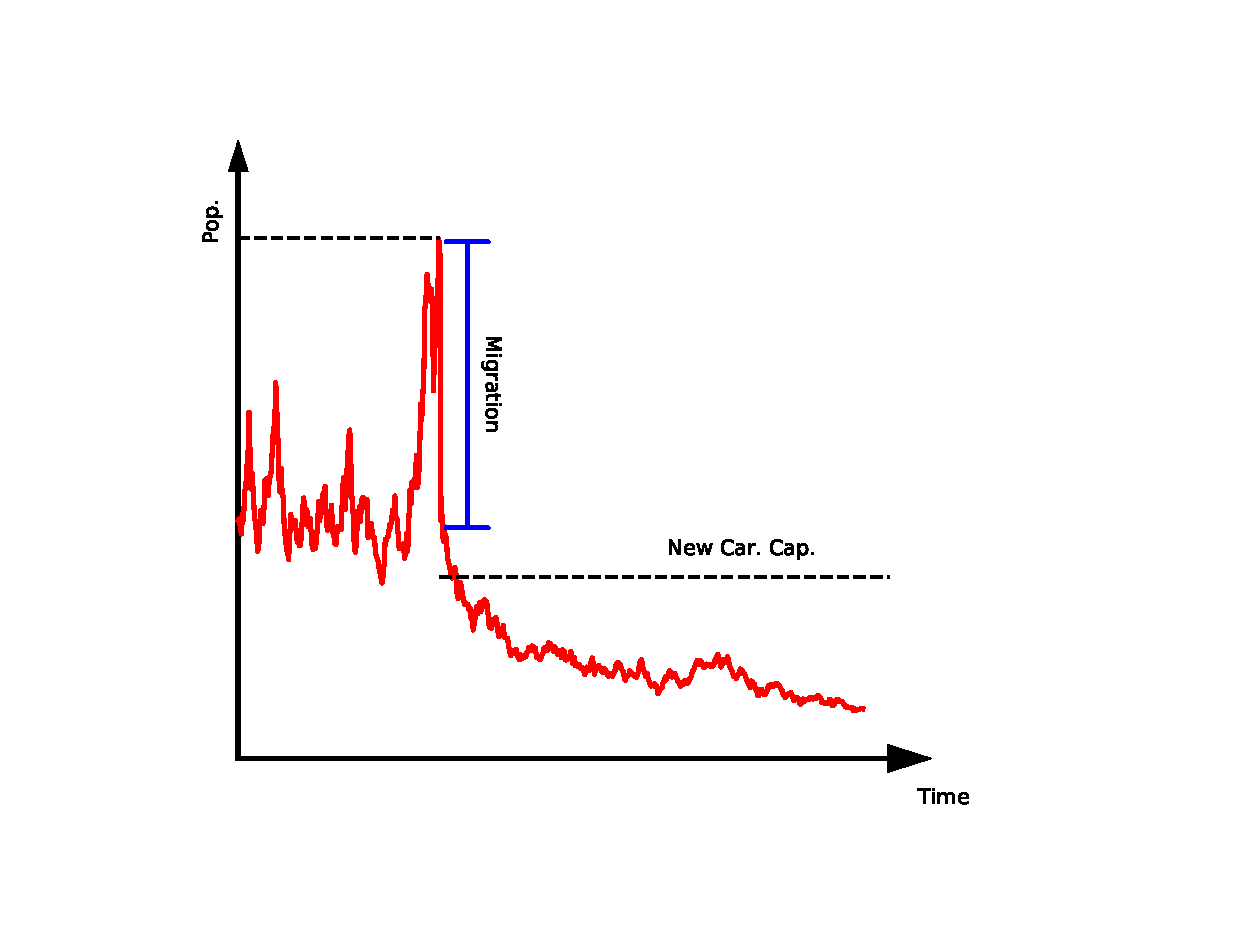
\includegraphics[width=\textwidth]{AncillaryFiles//figure25.eps}
\caption{An illustration of the formation of a phylogenetic tree. The left-hand side of the figure denotes times at which the barrier is hit, triggering mass migrations. Note that the length of the tree corresponds with the length of the path starting at $A$, which is also the same as the sums of the other branches.} \label{evo0}
\end{center} 
\end{figure}





\footnote{This has yet to be shown and this part of the paper is weak.} The result of these ideas is something like figure \ref{evo1}. The figure shows mean-reverting processes eventually hitting an upper limit, which resets the process and produces a migratory event. This sequence of events continues at the next location. The idea behind the process is illustrated in figure \ref{evo1}.

\begin{figure}
\begin{center}
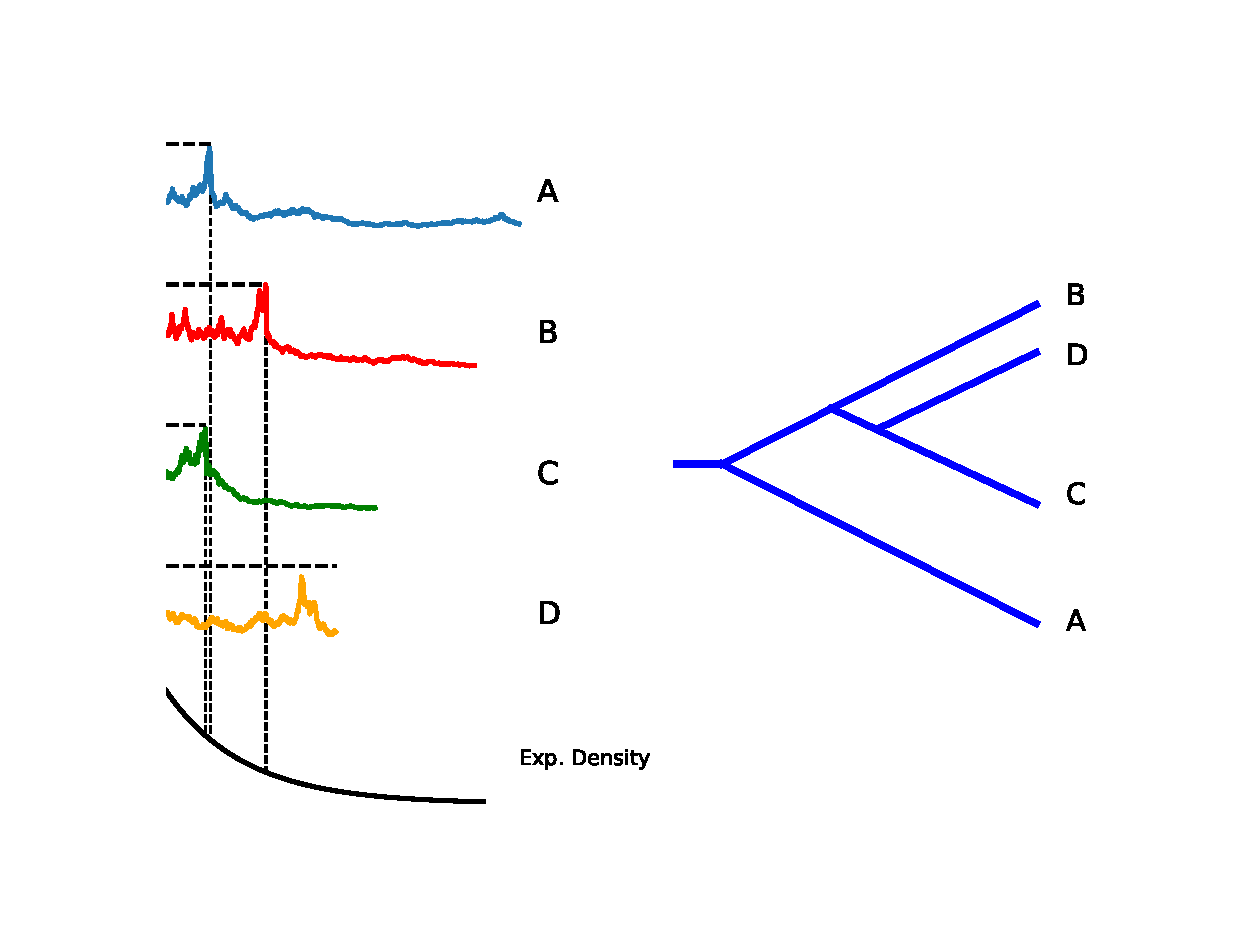
\includegraphics[width=\textwidth]{AncillaryFiles//figure3.eps}
\caption{An illustration of the formation of a phylogenetic tree. The left-hand side of the figure denotes times at which the barrier is hit, triggering mass migrations. Note that the length of the tree corresponds with the length of the path starting at $A$, which is also the same as the sums of the other branches.} \label{evo1}
\end{center} 
\end{figure}


\section{Computation}

In this section I  show how one can couple choice of the optimal path through a tree by working recursively back through the tree, employing a dynamic programming algorithm to obtain the probability that all points in the tree were the geographic point of origin of the tree. First, imagine that all interior nodes have been enumerated in depth-first order, so that nodes nearer to leaves or taxa carry lower indices. This allows a backwards traversal of the tree via the index. Both the trees in \ref{fig1} and \ref{ex1} have followed this convention. 

Label interior nodes along the tree $v=1,2,3,\hdots,V$, with terminal branches carrying their `names'  $k=1,2,3,\hdots,K$. 
I can now recursively develop an expression for the probability that location $k$ is the origin for the family of cultures after having traversed the $v$th node, and once the root node is reached, there will be a full complement of probabilities associated with the hypothesis that $k$ was the point of origin. I begin by treating the case in which branch lengths are known, as the case in which they are not known can be handled by appropriate normalization of branch lengths. 
Let $L^*_{v,k}$ denote the likelihood that $k$ is the point of origin after considering the subtree spanned by node $v$. This is the maximal probability migratory history emanating from group $k$'s location, given the subtree starting at $v $. Let $t_{kv}$ denote the length of a chain starting at node $v$ given it emanated from $k$'s location.  


I useful introduce the notion of the \textit{descendants} of node $v$. These are all the terminal nodes that can be reached from a directed path starting at node  $v$, proceeding to the roots. A related useful function is the function $A(i,v)$ - these are all of the descendant nodes that were not reachable from $k$ until node $v$ is considered.  

At $v=0$, the algorithm starts with $L_{k,0} =1$, and the two state variables $t_{k,0}=t_i$, and $n_{ik} = 0$, which are, respectively, the length of a branch and the number of jumps given a migratory chain starting at $k$. Now, define:
\begin{equation} \label{ca1}
t_{i,k}=t_k +\ t_j^*
, \quad t_j&*=\argmax_{j\in A(i,k)}\{t_j:j,f(t_j+t_k,n_i+1\right)\}
\end{equation}
and
\begin{equation*}
n_{ik+1}=n_{ik}+1
\end{equation*}
Further, define the conditional log-likelihood as:
\begin{equation*}\ln
L_{ik}^*= \ln L^*_{ik-1} + \ln(f(t_{ik},n_{ik}))
\end{equation*}

\subsection{An example}
As an example of how the algorithm works, consider the phylogenetic tree depicted in figure \ref{afig}.
\begin{figure}
\begin{center}
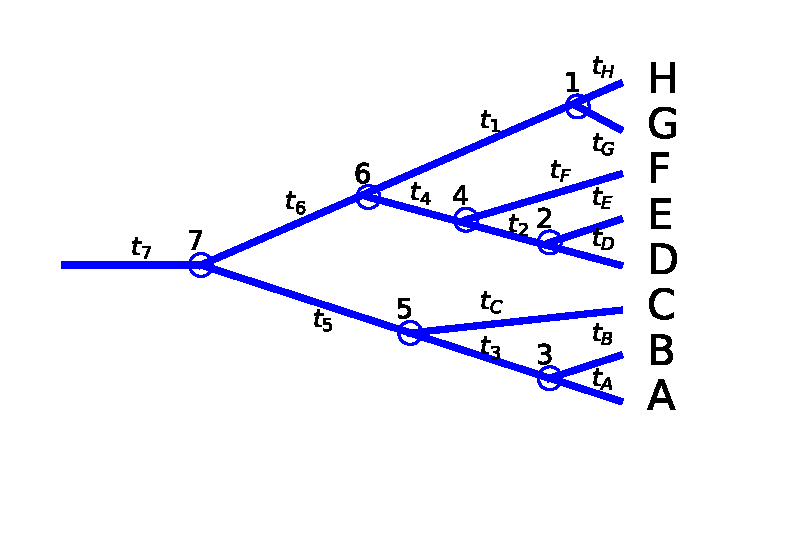
\includegraphics[width=\textwidth]{AncillaryFiles//algofig.eps}
\caption{An illustration of the formation of a phylogenetic tree. The left-hand side of the figure denotes times at which the barrier is hit, triggering mass migrations. Note that the length of the tree corresponds with the length of the path starting at $A$, which is also the same as the sums of the other branches.} \label{afig}
\end{center} 
\end{figure}

\begin{table}
\begin{center}
\begin{tabular}{lccc}
Culture & $t^*_3$ & $n_3$ & $LL_3$ \\
H& $t_1+t_G$ & 1 & 0 \\ 
G& $t_1+t_H$ & 1 & 0     \\
F& $t_F $    & 0 & 0                 \\
E& $t_2+t_D  & 1 & 0                   \\
D& $t_2+t_E  & 1 & 0                    \\ 
C& $t_c$      & 0 & 0                    \\
B& $t_3+t_A$ & 1 & 0                    \\
A& $t_3+t_B$ & 1 & 0                
\end{tabular} \caption{Algorithm at $k=3$}
\end{center}
\end{table} 


\begin{table}
\begin{center}
\begin{tabular}{lccc}
Culture & $t^*_3$ & $n_3$ & $LL_3$ \\
H& $t_1+t_G$ & 1 & 0 \\ 
G& $t_1+t_H$ & 1 & 0     \\
F& $t_4+t_2+t_D $    & 2 & 0                 \\
E& $t_4+t_F  & 1 & $-\ln(t_2+t_E ) $                 \\
D& $t_4+t_F  & 1 & $-\ln(t_2+t_E)$                    \\ 
C& $t_5+t_3+t_B$      & 2 & 0                    \\
B& $t_5+t_C$ & 1 &  $-\ln(t_3+t_A) $                   \\
A& $t_5+t_C$ & 1 &  $- \ln(t_3+t_B)$                
\end{tabular} \caption{Algorithm at $k=5$}
\end{center}
\end{table} 
\begin{table}
\begin{center}
\begin{tabular}{lccc}
Culture & $t^*_6$ &$ n_6$ & $LL_6$ \\
H& $t_6+t_4+t_2+t_D$ & 1 & $-\ln(t_1+t_G)$ \\ 
G& $t_6+t_4+t_2+t_D$ & 1 & $- \ln(t_1+t_H)$     \\
F& $t_6+t_1+t_H $    & 2 & $2(\ln2-\ln(t_4+t_2+t_D))$                \\
E& $t_6+t_1+t_H  & 1 & $-\ln(t_4+t_F)-\ln(t_2+t_D )$                  \\
D& $t_6+t_1+t_H & 1 & $-\ln(t_4+t_F)-\ln(t_2+t_E)$                    \\ 
C& $t_5+t_3+t_B$      & 2 & 0                    \\
B& $t_5+t_C$ & 1 & $ -\ln(t_3+t_A) $                   \\
A& $t_5+t_C$ & 1 & $ - \ln(t_3+t_B)$                
\end{tabular} \caption{Algorithm at $k=6$}
\end{center}
\end{table} 

\begin{table}
\begin{center}
\begin{tabular}{lccc}
Culture  & $t^*_7$ & $n_7$ &$LL_7$ \\
H& $t_7+t_5+t_3+t_B$ & 3 & $3(\ln3-\ln(t_6+t_4+t_2+t_D))-\ln(t_1+t_G)$ \\ 
G& $t_7+t_5+t_3+t_B$ & 3 & $3(\ln3-\ln(t_6+t_4+t_2+t_D))- \ln(t_1+t_H)$     \\
F& $t_7+t_5+t_3+t_B $    & 3 & $2(\ln2-\ln(t_6+t_1+t_H))+2(\ln2-\ln(t_4+t_2+t_D))$                 \\
E& $t_7+t_5+t_3+t_B$  & 3 & $2(\ln 2-\ln(t_6+t_1+t_H)-\ln(t_4+t_F)-\ln(t_2+t_D )$                  \\
D& $t_7+t_5+t_3+t_B$ & 3&$2(\ln2-\ln(t_6+t_1+t_H)-\ln(t_4+t_F) -\ln(t_2+t_E)$                    \\ 
C& $t_7+t_6+t_4+t_2+t_E$      & 4 &$ 2(\ln2-\ln(t_5+t_3+t_B)            $        \\
B& $t_7+t_6+t_4+t_2+t_E$ & 4 &  $-\ln(t_5+t_C)-\ln(t_3+t_A)  $                  \\
A& $t_7+t_6+t_4+t_2+t_E$ & 4 &  $-\ln(t_5+t_C)- \ln(t_3+t_B)$                
\end{tabular} \caption{Algorithm at $k=7$}
\end{center}
\end{table} 

\begin{table}
\begin{center}
\begin{tabular}{lc}
Culture & Log-likelihood \\
H& $3(\ln(3)-\ln(t_7+t_5+t_3+t_B)) + 3(\ln3-\ln(t_6+t_4+t_2+t_D))-\ln(t_1+t_G)$ \\ 
G& $3(\ln(3)-\ln(t_7+t_5+t_3+t_B))+3(\ln3-\ln(t_6+t_4+t_2+t_D))- \ln(t_1+t_H)$     \\
F& $3(\ln(3)-\ln(t_7+t_5+t_3+t_B)) +2(\ln2-\ln(t_6+t_1+t_H))+2(\ln2-\ln(t_4+t_2+t_D))$                 \\
E& $3(\ln(3)-\ln(t_7+t_5+t_3+t_B))+2(\ln 2-\ln(t_6+t_1+t_H)-\ln(t_4+t_F)-\ln(t_2+t_D )$                  \\
D& $3(\ln(3)-\ln(t_7+t_5+t_3+t_B))+2(\ln2-\ln(t_6+t_1+t_H)-\ln(t_4+t_F) -\ln(t_2+t_E)$                    \\ 
C& $4(\ln(4)-\ln(t_7+t_6+t_4+t_2+t_E))+ 2(\ln2-\ln(t_5+t_3+t_B)            $        \\
B& $4(\ln(4)-\ln(t_7+t_6+t_4+t_2+t_E))-\ln(t_5+t_C)-\ln(t_3+t_A)  $                  \\
A& $4(\ln(4)-\ln(t_7+t_6+t_4+t_2+t_E))-\ln(t_5+t_C)- \ln(t_3+t_B)$              
\end{tabular} \caption{Algorithm at conclusion, known branch lengths. Poisson model can be recovered by replacing time terms with factorials.}
\end{center}
\end{table} 


\section{Extensions}

\subsection{Approximations}

Using Stirling's approximation, one can write the likelihood very simply, which relates the jump method to simple counting. 

\subsection{Additional information}

One can also modify the model to include explicit information about distance and space. One possibility is to do this in such a way so as to reflect that moving larger distances is less likely, and many analyses commonly include such spatial features.

\subsection{Expanded likelihoods}
There are many ways in which the model can be extended. Since a dynamic programming algorithm lies at the heart of the analysis, one can in principle include any number of things in the optimization decision.  A prominent possibility  is physical distance. As alluded to above, when equipped with a model producing a likelihood, one can bind this to other components of a likelihood. 

For example, one possible idea is to interpret the likelihood presented in the previous few pages as a conditional likelihood, and incorporate it into a joint estimation procedure. For example, if one has a means of computing the likelihood of a particular tree, one can then think about the joint distribution of a likelihood and a tree at the same time using the simple probabilistic relationship:
$$
P(\mathcal{T},\mathcal{H})=P(\mathcal{H}|\mathcal{T})P(\mathcal{T})
$$
This is important because th
ere are so many methods for computing the likelihood of a given linguistic tree. This allows one to consider a migratory route as part of the estimation process, rather than just something loosely implied by the structure of the tree. One can also form a picture of the distribution of trees and roots once one is equipped with a likelihood function. 

Another important facet is the ability to include information for other sources, as in a Bayesian analysis. 

\subsection{Including additional information about migrations}

Part of the optimization relationship can also include additional information about what routes are more likely. As one example, one might include a matrix of physical distances or travel costs between points. This matrix might even reflect.\footnote{If one is interested, computational algorithms and extensions can be found on the project site:} 

\section{Applications}

\subsection{Afroasiatic}

\subsection{Na Dene}

\section{Conclusions}


\newpage
\bibliographystyle{apalike}
\bibliography{bibfile}

\end{document} 
